% ********** Chapter 5 **********
\chapter{(2,4)-boom}
\label{sec:Hoofdstuk 5}

\begin{figure}[h]
	\centering
		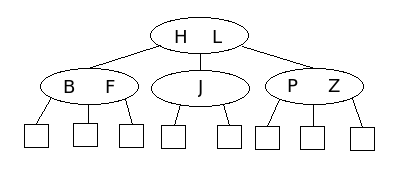
\includegraphics[width=\textwidth]{chap5/24tree}
	\label{fig:24tree}
\end{figure}

\section{Introductie}
De tweede gebalanceerde boom die behanded wordt is de (2,4)-boom. Alle interne knopen van deze boom hebben ��n tot drie keys, het aantal kinderen van een knoop is het aantal keys + 1. Dit betekent dus dat elke knoop 2, 3 of 4 kinderen heeft, vandaar de naam (2,4)-boom (soms ook (2,3,4)-boom genoemd). Een andere eigenschap van deze boom is dat de diepte van alle externe knopen gelijk is. Deze eigenschappen zorgen ervoor dat de hoogte van een (2,4)-boom met $n$ items $\Theta(log n)$ is. Deze eigenschappen worden bewaard door na elke toevoeging of verwijdering te kijken of de boom gebalanceerd moet worden. De boom moet gebalanceerd worden wanneer een knoop in de boom geen keys (woorden) meer bevat of wanneer een knoop meer dan drie keys bevat.\\
\\
\section{Balanceren}
Omdat bij deze analyse alleen gekeken wordt naar het toevoegen van keys zal de boom alleen gebalanceerd worden wanneer een knoop meer dan drie keys bevat. Wanneer een knoop meer dan drie keys bevat (overflow), zal de boom gebalanceerd moeten worden.
Dit wordt gedaan door de derde waarde van de knoop met meer dan drie keys toe te voegen aan zijn parent. De eerste twee keys worden dan het kind aan de linkerkant van toegevoegde key in de parent en de vierde waarde het kind aan de rechterkant.\\
\\
\section{Zoeken}
Bij het zoeken van een key zal begonnen worden bij de root knoop. Als de knoop niet de gezochte key bevat zal gekeken worden in het kind aan de linkerkant van de key die lager is dan de invoer. Dit wordt gedaan tot een externe knoop is bereikt of tot een knoop is bereikt die de invoer bevat.\\
\\
\section{Toevoegen}
Bij het toevoegen zal eerst gezocht worden op de bovenstaande manier. Wanneer een knoop wordt gevonden die de key al bevat zal gestopt worden met toevoegen. Als dit niet het geval is, we hebben dan dus een externe knoop, zal de waarde toegevoegd worden aan de parent. Hierna zal de balance methode aangeroepen worden om te kijken of de boom ongebalanceerd is en balanceren wanneer dit het geval is.\\
\\
\section{Analyse}


% ********** End of chapter **********